\clearpage
\section{Diagramas de Casos de Uso}
\label{sec:casos_uso}

A continuación se presentan los diagramas de casos de uso correspondientes a los tres requerimientos funcionales (RQF-03, RQF-04 y RQF-05) descritos en la sección de Requerimientos Funcionales. Los requerimientos no funcionales no se diagraman por tratarse de cualidades transversales del sistema y no de interacciones discretas del usuario.

\subsection{RQF-03 — Anti-spam y validación de email}

El siguiente diagrama describe la interacción del usuario con cualquiera de los formularios de autenticación (inicio de sesión, registro o recuperación de contraseña). La validación local previene el envío de peticiones HTTP con datos malformados y el bloqueo del botón impide envíos duplicados.

\begin{figure}[h!]
  \centering
  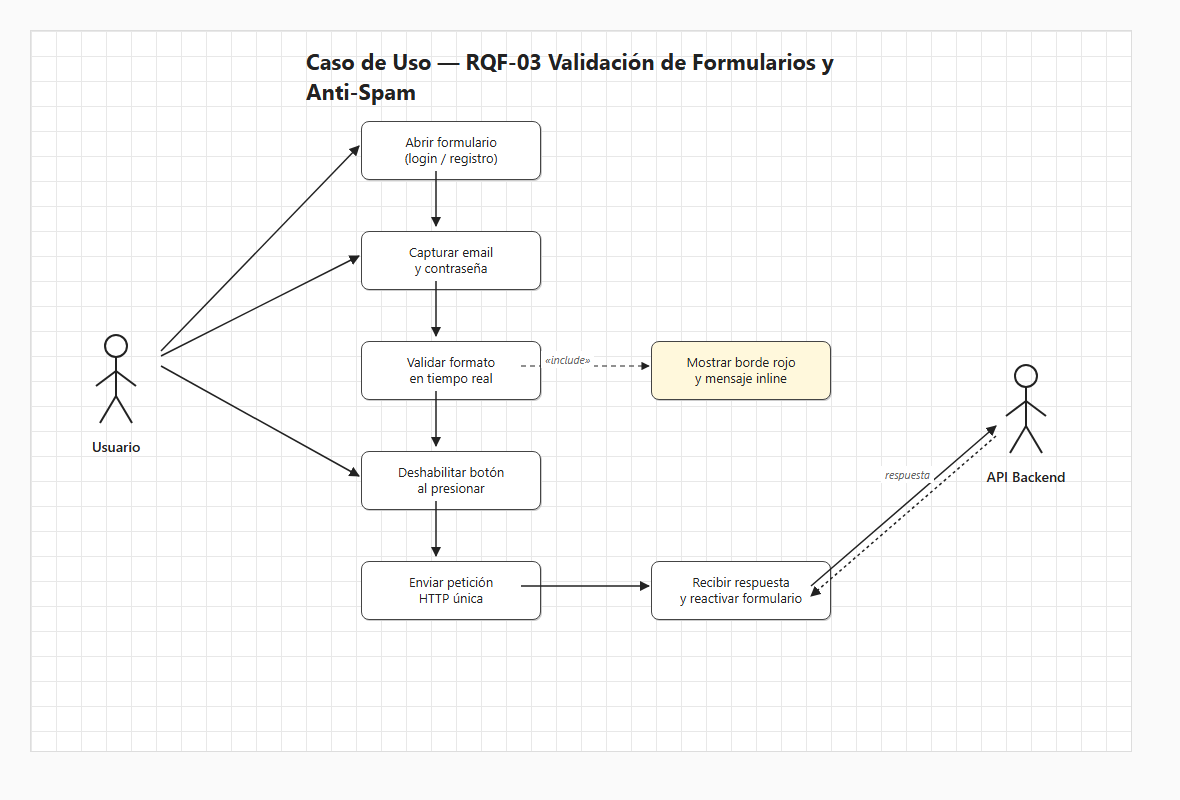
\includegraphics[width=0.85\textwidth]{images/rqf03_validacion.png}
  \caption{Diagrama de casos de uso — Validación de formularios y anti-spam}
\end{figure}

\subsection{RQF-04 — Indicador de conexión y caché offline}

El siguiente diagrama describe el comportamiento del dashboard al detectarse un cambio en la conectividad del dispositivo. El sistema decide entre mostrar datos en vivo, datos cacheados o un banner informativo según el estado de la red.

\begin{figure}[h!]
  \centering
  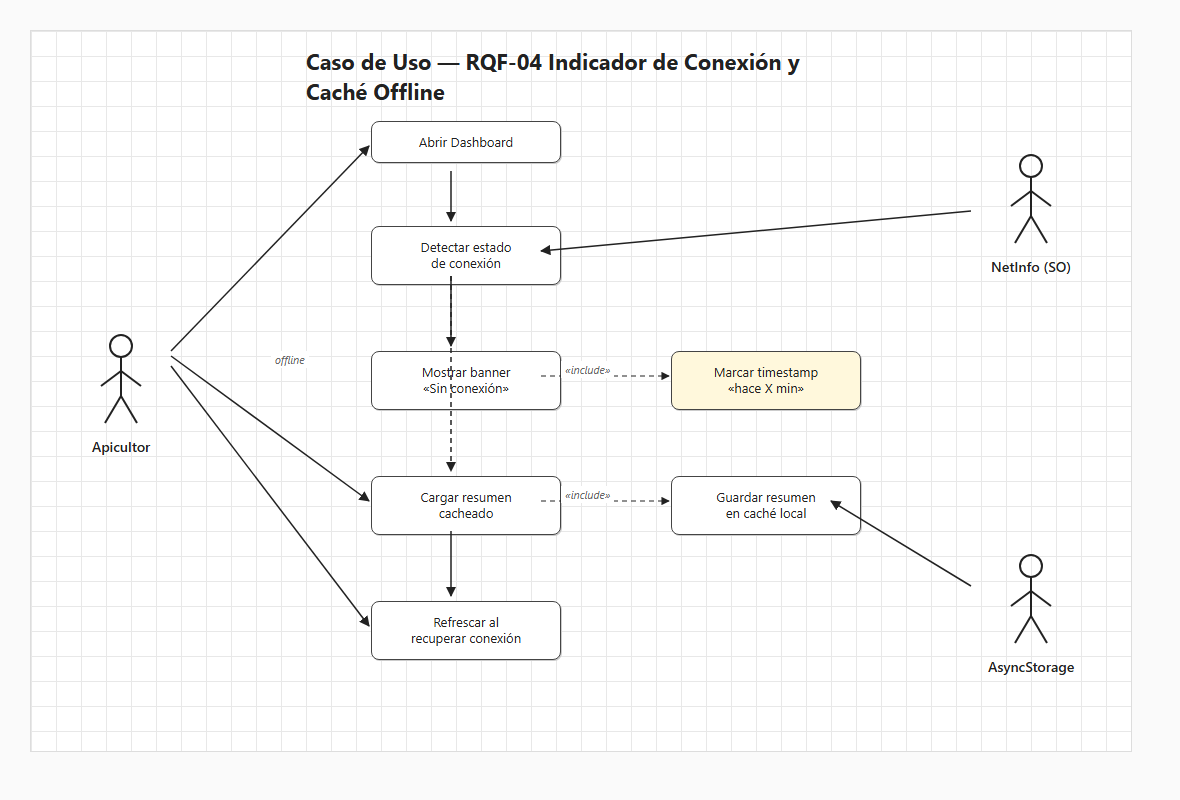
\includegraphics[width=0.85\textwidth]{images/rqf04_offline.png}
  \caption{Diagrama de casos de uso — Indicador de conexión y caché offline}
\end{figure}

\clearpage
\subsection{RQF-05 — Bitácora apícola con calendario}

El siguiente diagrama describe las interacciones del apicultor con la nueva pantalla de bitácora y con el acceso rápido desde la pantalla de detalle de colmena. Ambos puntos de entrada culminan en la persistencia del evento en el backend.

\begin{figure}[h!]
  \centering
  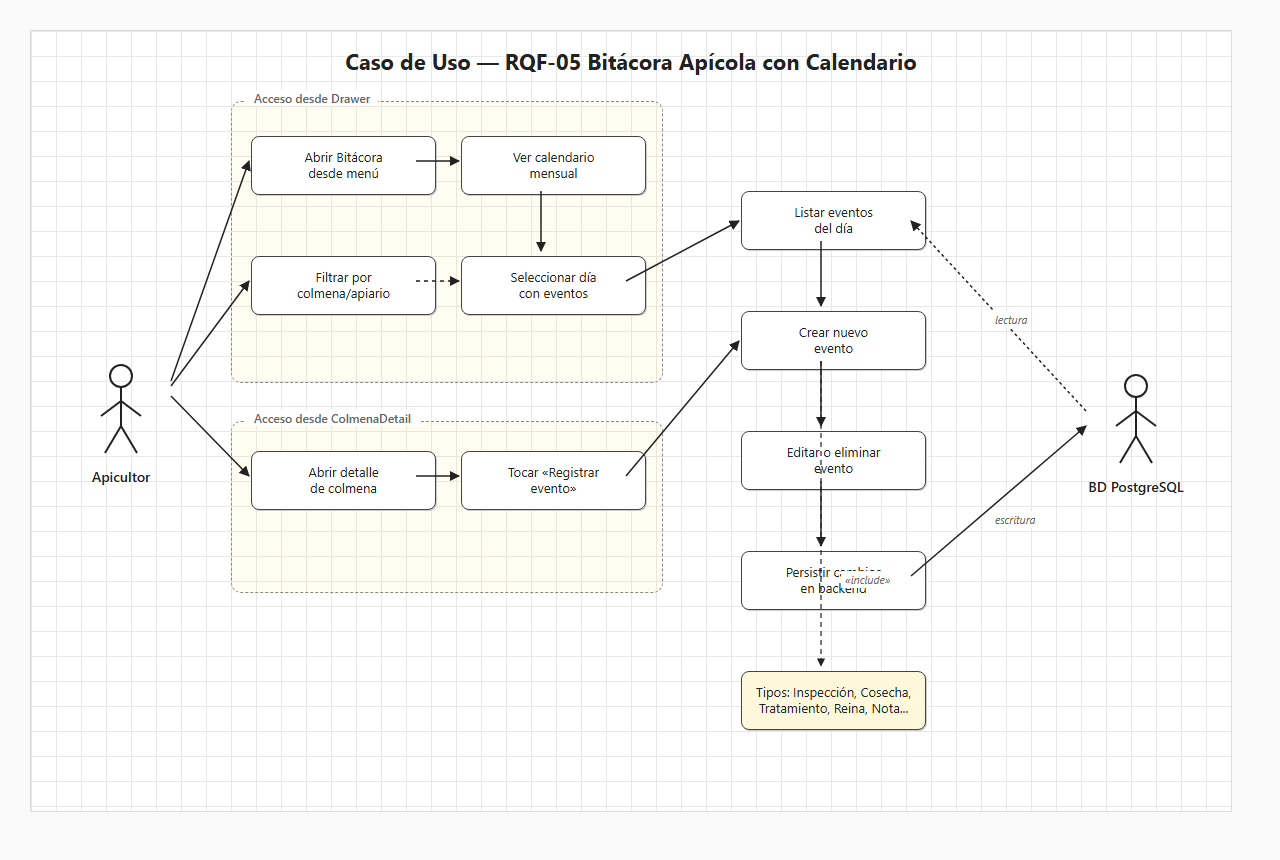
\includegraphics[width=0.95\textwidth]{images/rqf05_bitacora.png}
  \caption{Diagrama de casos de uso — Bitácora apícola con calendario}
\end{figure}

\subsection{Priorización MoSCoW}

\begin{table}[h!]
\centering
\caption{Priorización de los nuevos requerimientos}
\renewcommand{\arraystretch}{1.2}
\begin{tabular}{@{}lp{10cm}@{}}
\toprule
\textbf{Prioridad} & \textbf{Requerimientos} \\
\midrule
\textbf{Must have} & RQF-03 (anti-spam y validación), RQF-04 (caché offline), RNF-03 (bloqueo por inactividad) \\
\textbf{Should have} & RQF-05 (bitácora apícola), RNF-01 (soporte bilingüe), RNF-02 (háptico y toasts) \\
\textbf{Could have} & RNF-04 (compatibilidad multiplataforma validada), RNF-05 (rendimiento $<$ 2s medido y documentado) \\
\textbf{Won't have} & Rediseño visual integral, soporte para wearables/Smart TV e integración con pagos, mapas o IA (fuera del alcance de esta iteración) \\
\bottomrule
\end{tabular}
\end{table}
